 \begin{figure}[h!]
\centering
 \subfloat[HR=2]{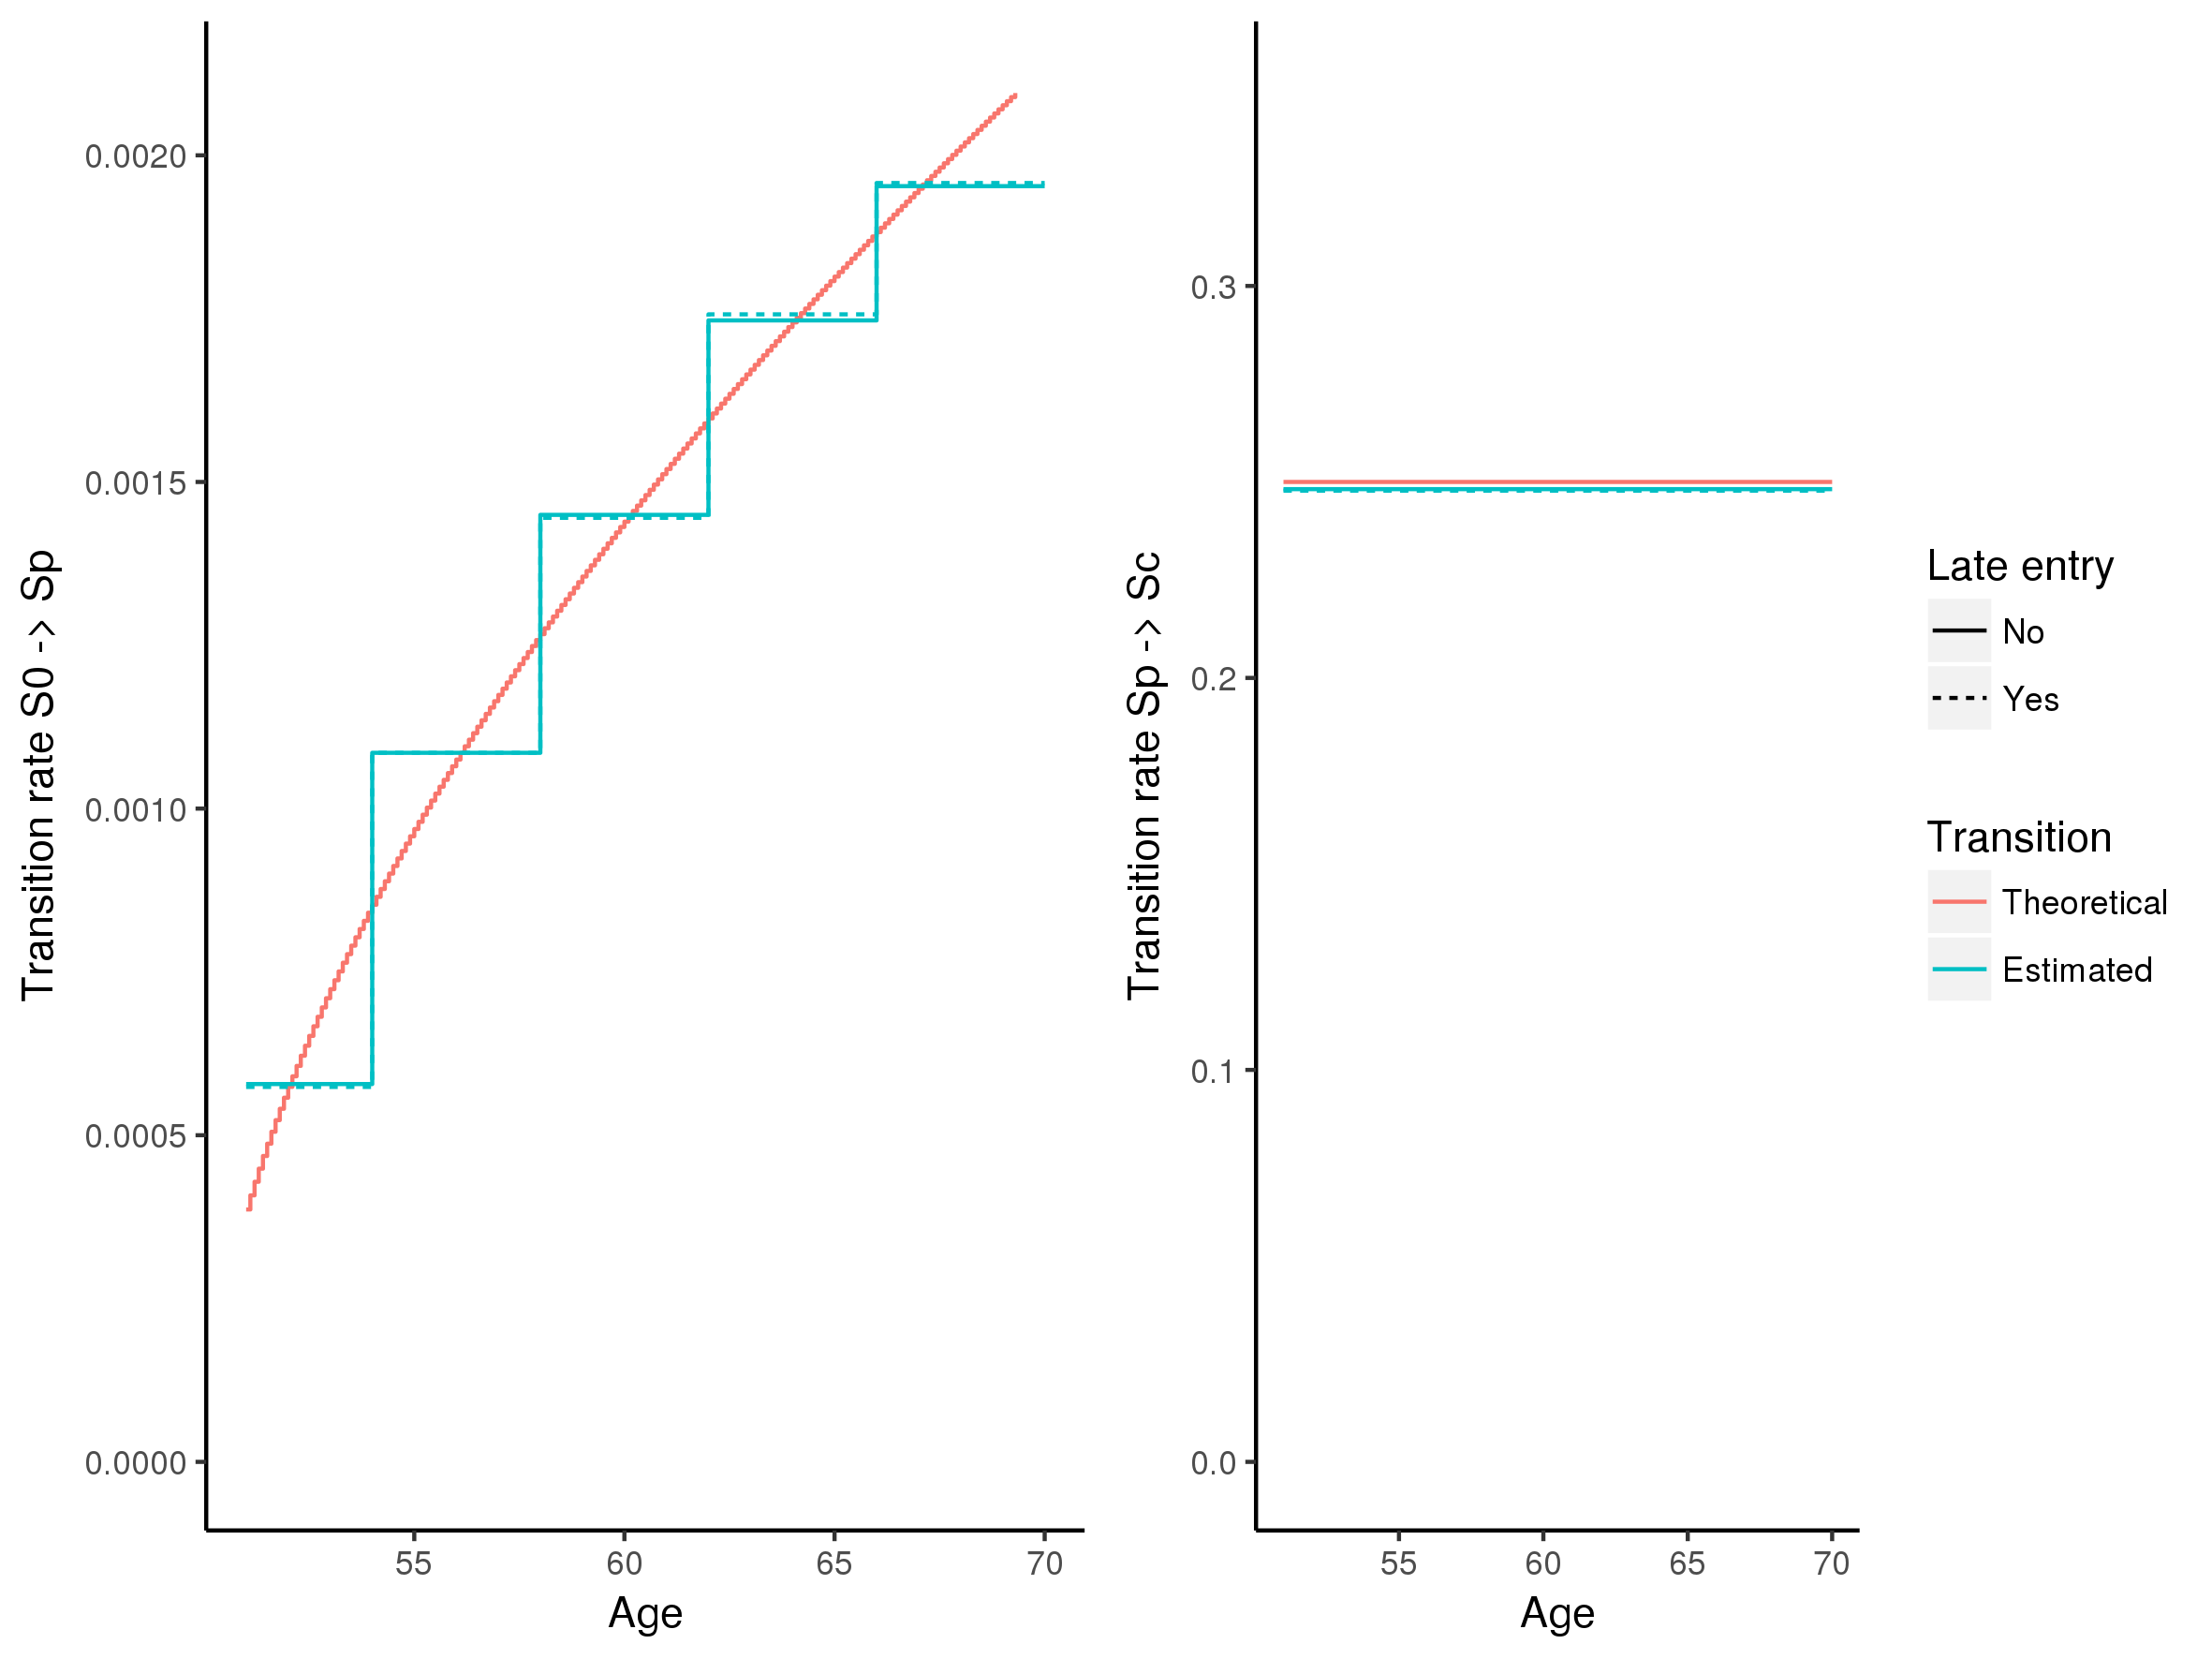
\includegraphics[width=0.7\textwidth]{fig/fig_1.png}}
 %\subfloat[HR=2]{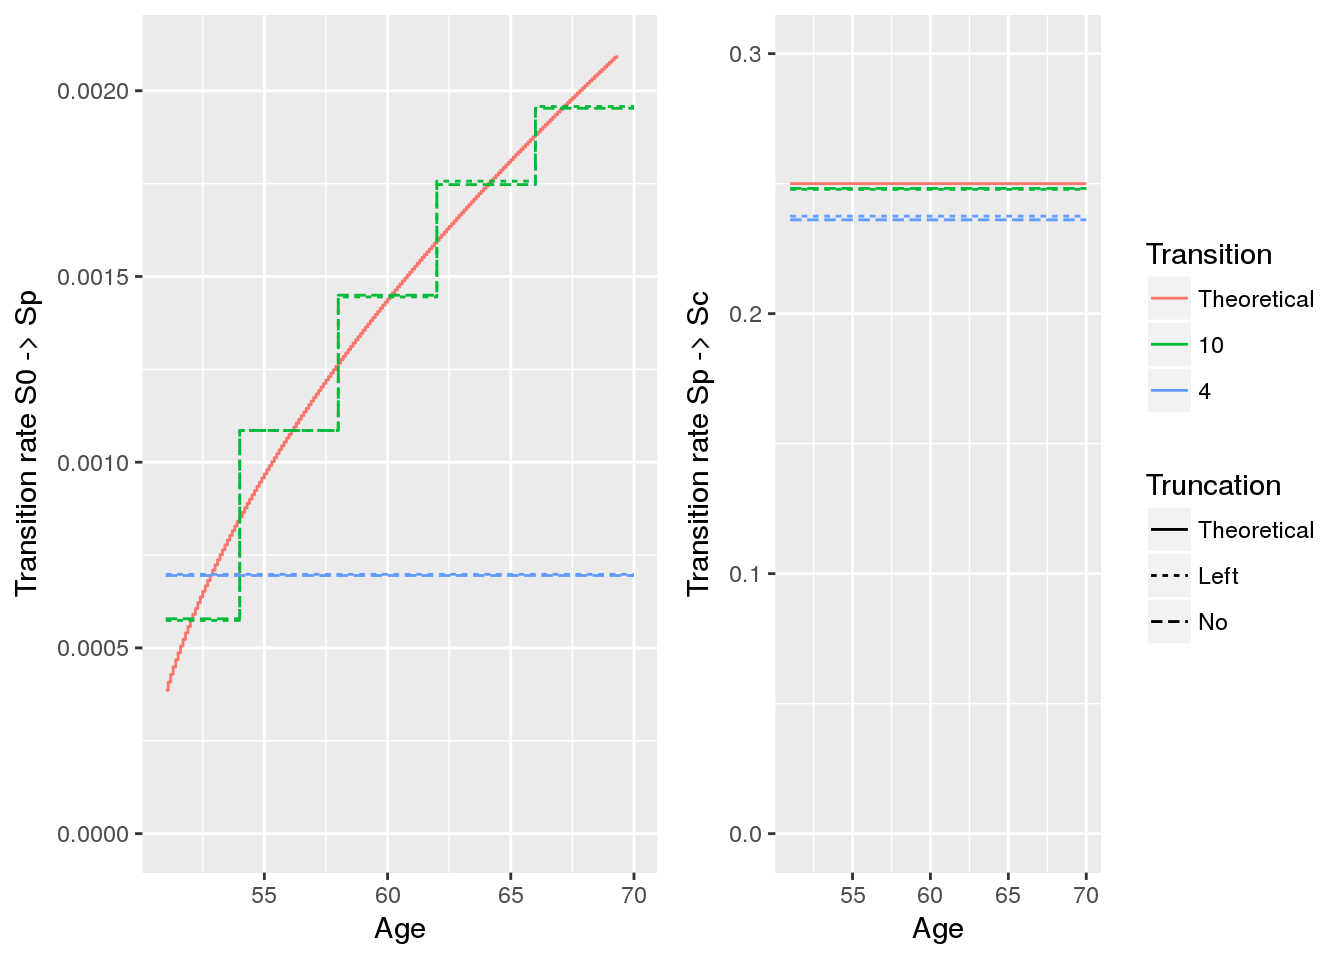
\includegraphics[width=0.7\textwidth]{fig/Fig_com_FP_HR_2.png}}

\caption{Transition intensities for the multi-state with three states (MS3) model. Complete data.}
\label{fig:trans_complete}
\end{figure}

 \begin{figure}[h!]
\centering
 \subfloat[HR=2]{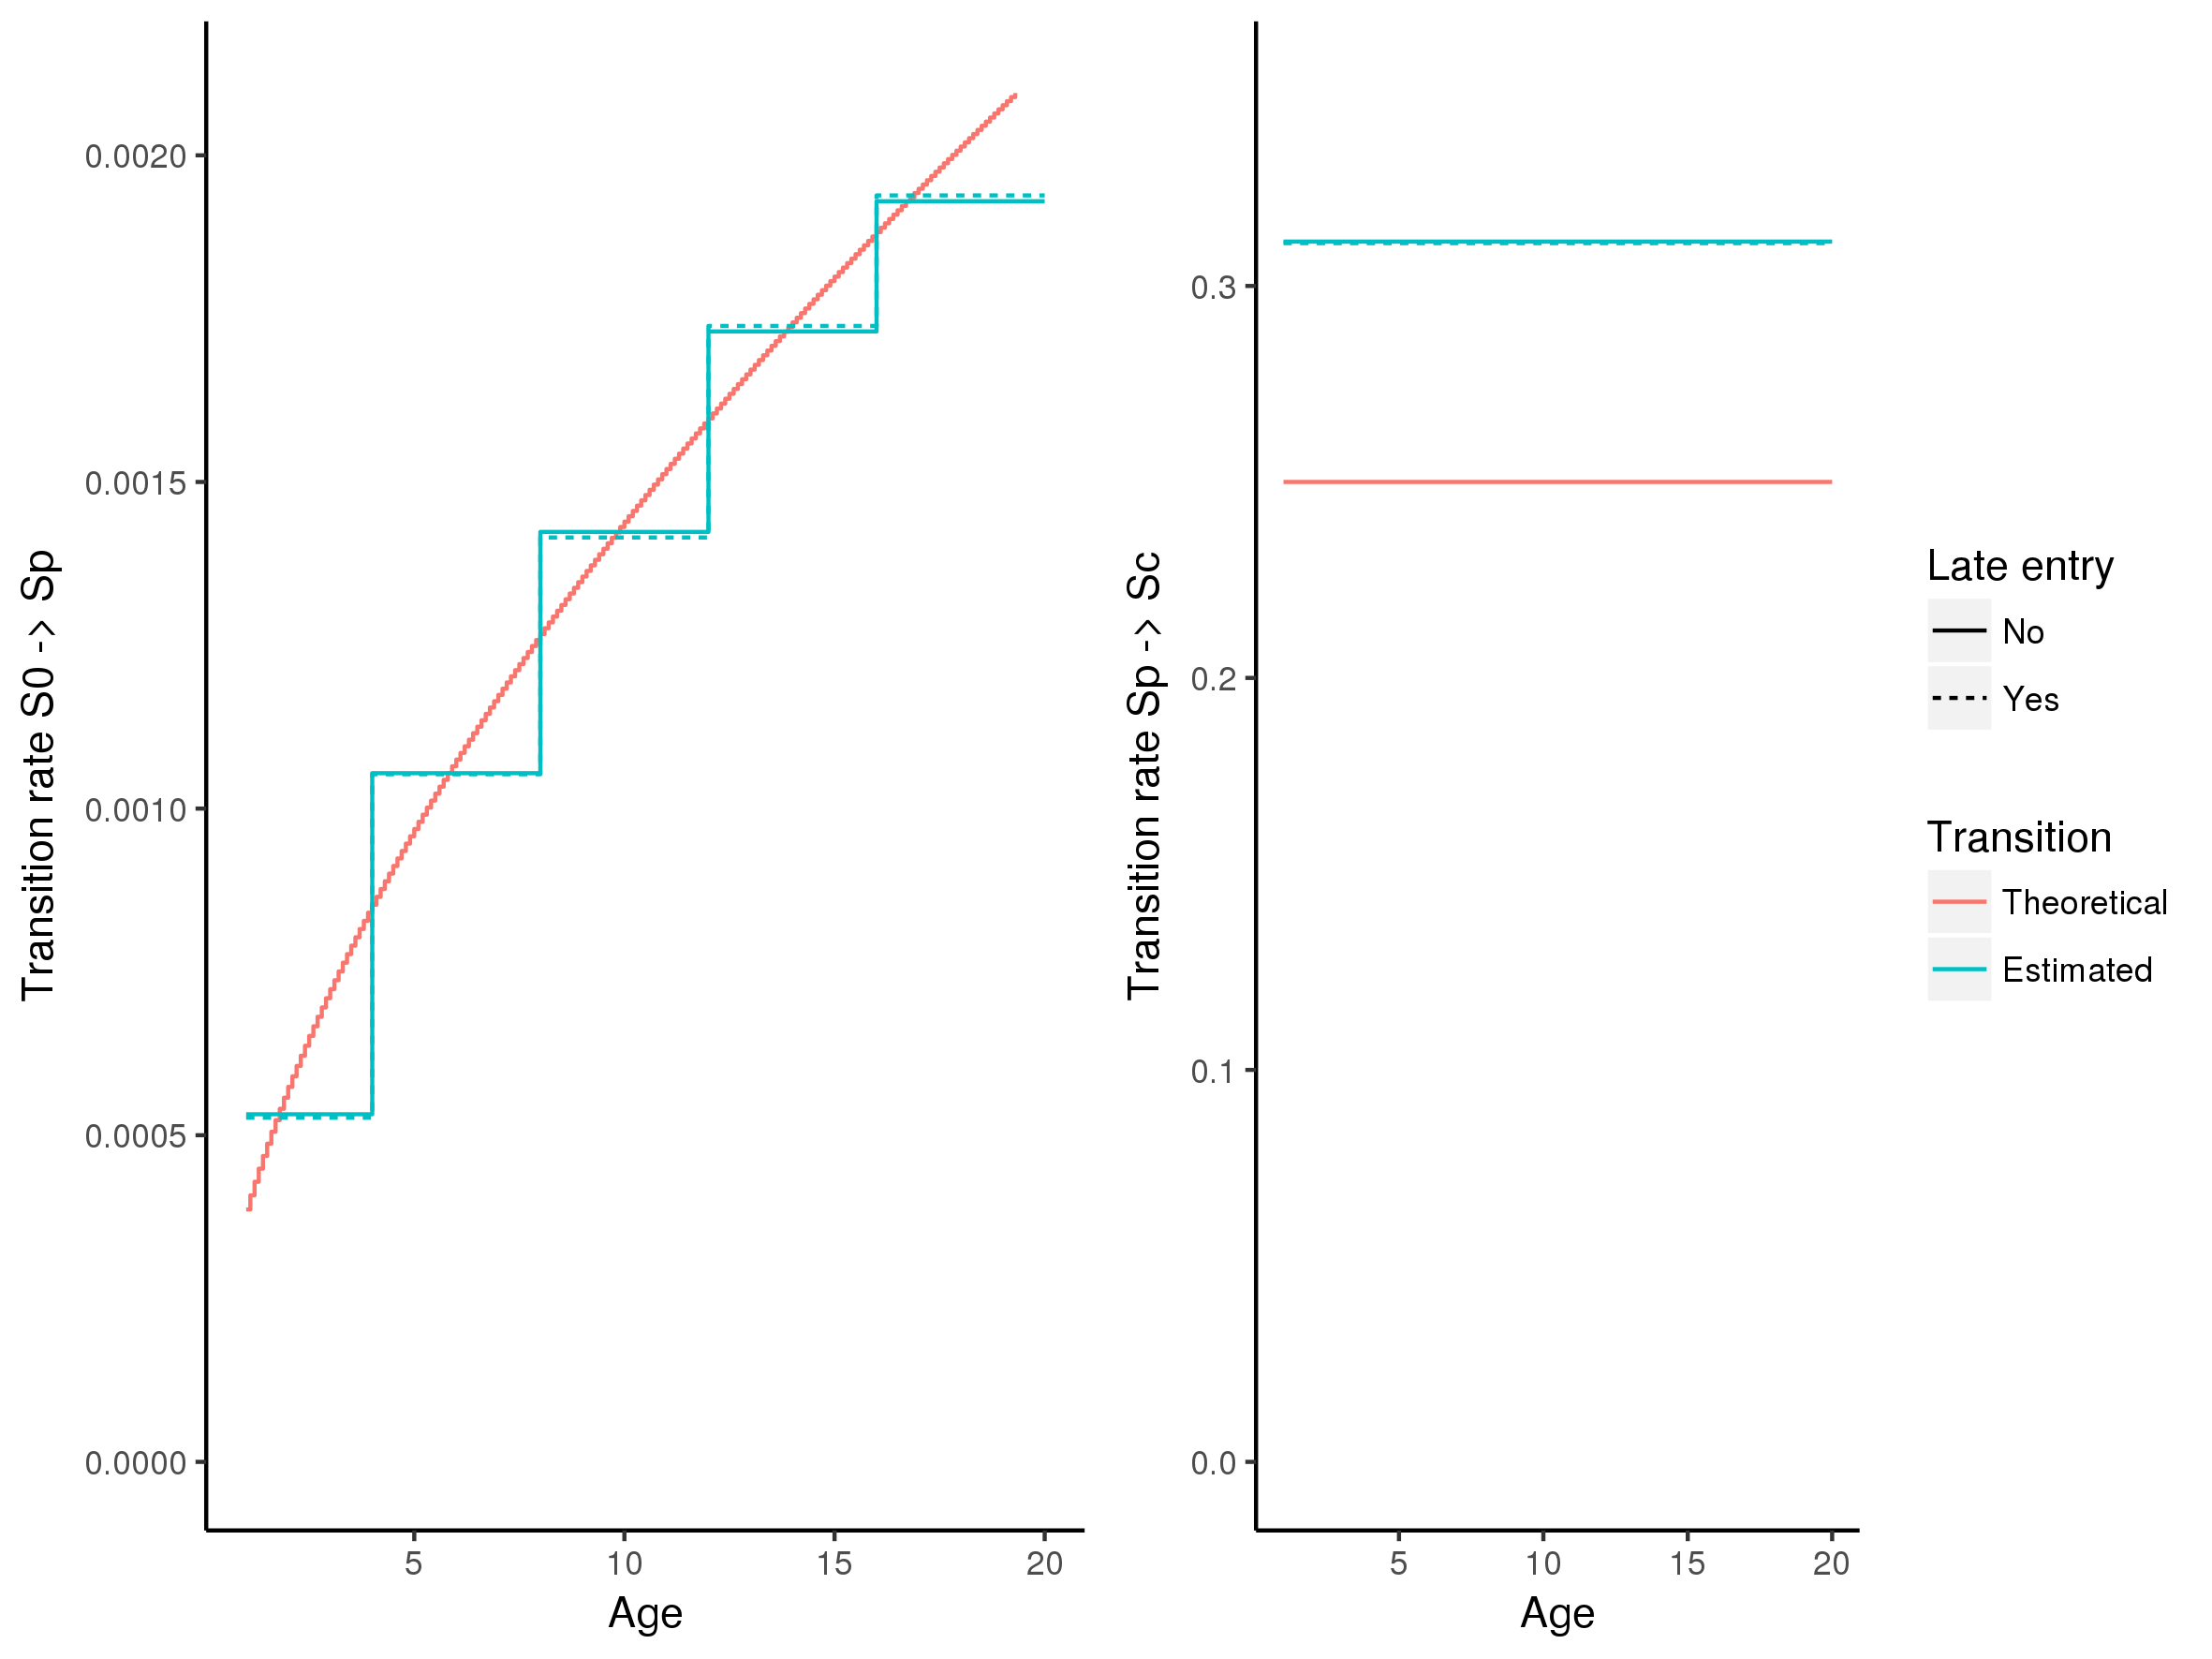
\includegraphics[width=0.7\textwidth]{fig/fig_2.png}}
% \subfloat[HR=2]{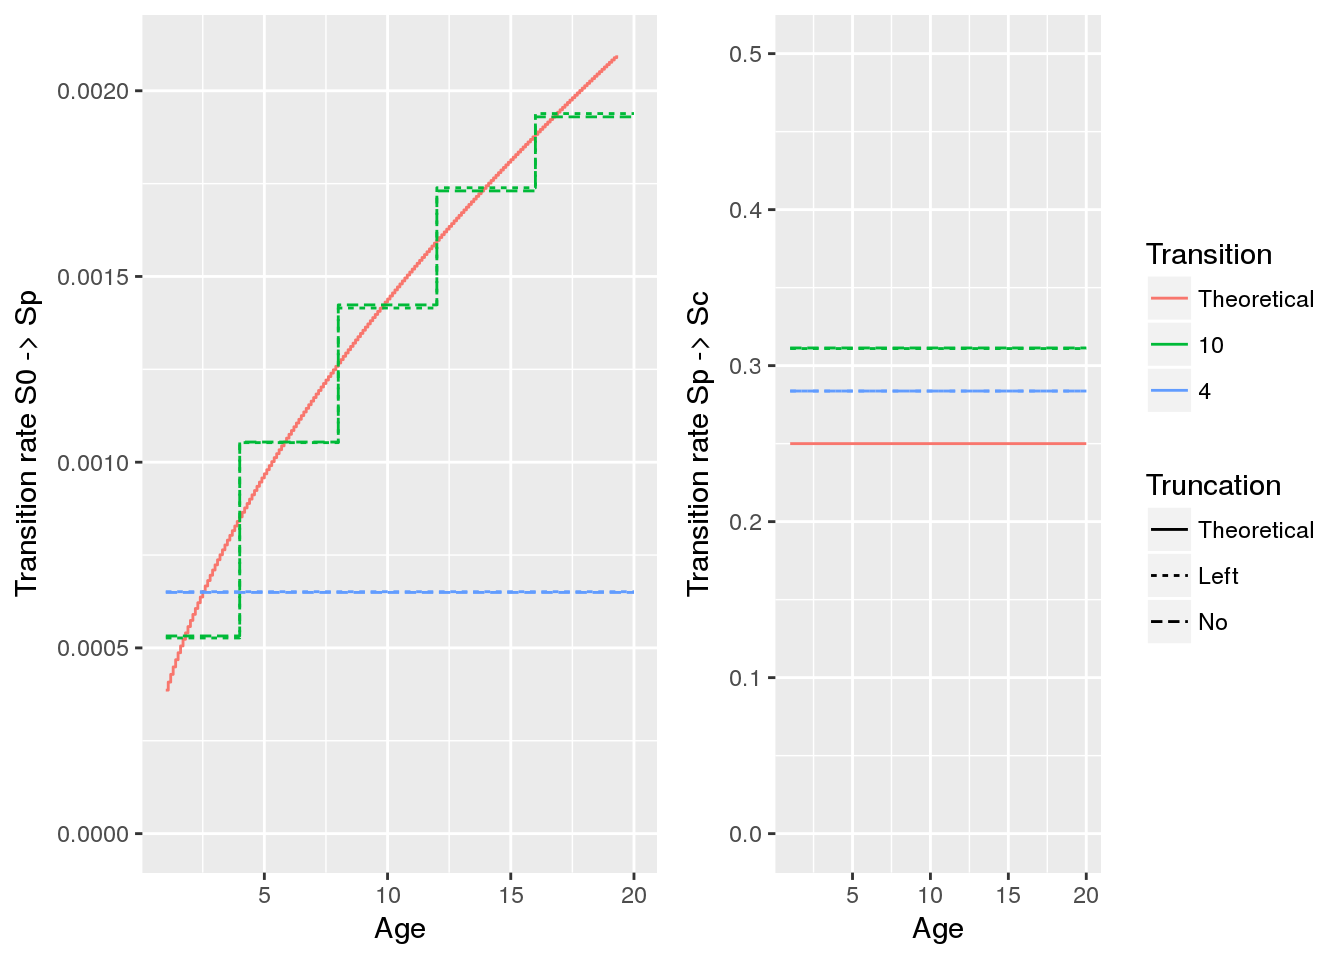
\includegraphics[width=0.7\textwidth]{fig/Fig_obs_FP_HR_2.png}}

\caption{Transition intensities for the multi-state with three states (MS3) model. Observed data.}
\label{fig:trans_observed}
\end{figure}




